\chapter{Design}

\section{Overall System Design}

\subsection{Short description of the main parts of the system}

\begin{itemize}
\item Log In Window
\item Main Database Interface
\item Adding/Removing/Editing Customers and Entries
\item Calender Interface
\item Changing Password

\item Search Window
\end{itemize}


\begin{itemize}
    \item Log In Window
    \begin{itemize}
        \item A window is displayed which prompts the user to input their ID and password.
        \item Checks the entered valiues with the database to identify whether the user's credentials are correct.
        \item Once a correct set of values are entered, the user will be granted access to the database.
        \item A link will be at the bottom which says "Forgotten password?". This can be clicked on and then the user wil be prompted for the email address, and the corresponding password for the email address entered will be sent to that email.
    \end{itemize}
  
    \item Main Database Interface
    \begin{itemize}
        \item This will be the "home" interface.
        \item A user interface is presented with a set of options which are: Search Database, Add Entry, Remove Entry, Edit Entry, Change Password, and Log out.
        \item Clicking the Search Database Button will prompt a seperate interface to open, and shows details which can be used to search for specific items in the database.
    \end{itemize}

    \item Adding/Removing/Editing Customers and Entries
    \begin{itemize}
        \item If a customer already exists, and details are needed to be added, edited, or deleted, a dropdown list will be available which will consist of existing customers, or alternatively an input box could be used for entering an Author's ID. 
        \item Clicking the Add Entry Button will prompt a seperate interface to open, and contains a layout of entry boxes for required fields for entering details about a new customer, or a book/royalties/royalty items/book invoice/book invoice items/publication invoice, dependent on which has been selected. An existing customer can be selected using the dropdown list or Author ID box if adding new details about an existing customer.
        \item Clicking the Remove Entry Button will prompt a seperate interface to open, which contains a view of the database. Entries can be searched for using the dropdown list or the Author ID box, and then can be selected and deleted.
        \item Clicking the Edit Entry button will prompt a seperate interface to open, and will contain a view of the database. An entry can be searched for using the dropdown list or the Author ID box, selected and once the user clicks "Edit", the window will be replaced by the window for Adding Entries, but the data will be in their respective entry fields already. Then, the data can be edited and saved.
    \end{itemize}

    \item Calendar Interface
    \begin{itemize}
        \item This interface will open when a date input is required. This will be when data is being searched for, or when data is being added or edited.
        \item It will consist of a visual calendar, and a date can be selected from clicking on a certain date.
        \item Once confirm is clicked, the selected date will be used for that entry.
    \end{itemize}

    \item Changing Password
    \begin{itemize}
        \item An interface will open, which will prompt the user to enter their Email, Old Password, and then the new password twice for confirmation.
        \item Once this has been confirmed, the interface will close, resorting back to the log in window.
    \end{itemize}
\end{itemize}


\subsection{System flowcharts showing an overview of the complete system}

\section{User Interface Designs}

\section{Program Structure}

\subsection{Top-down design structure charts}

\subsection{Algorithms in pseudo-code for each data transformation process}

\subsection{Object Diagrams}

\subsection{Class Definitions}

\section{Prototyping}

\section{Definition of Data Requirements}

\subsection{Identification of all data input items}

\subsection{Identification of all data output items}

\subsection{Explanation of how data output items are generated}

\subsection{Data Dictionary}

\subsection{Identification of appropriate storage media}


\newpage

\section{Database Design}

\subsection{Normalisation}
 
\subsubsection{ER Diagrams}


\begin{figure}[H]
    \caption{ER Diagram} \label{ER_Diagram.pdf}
    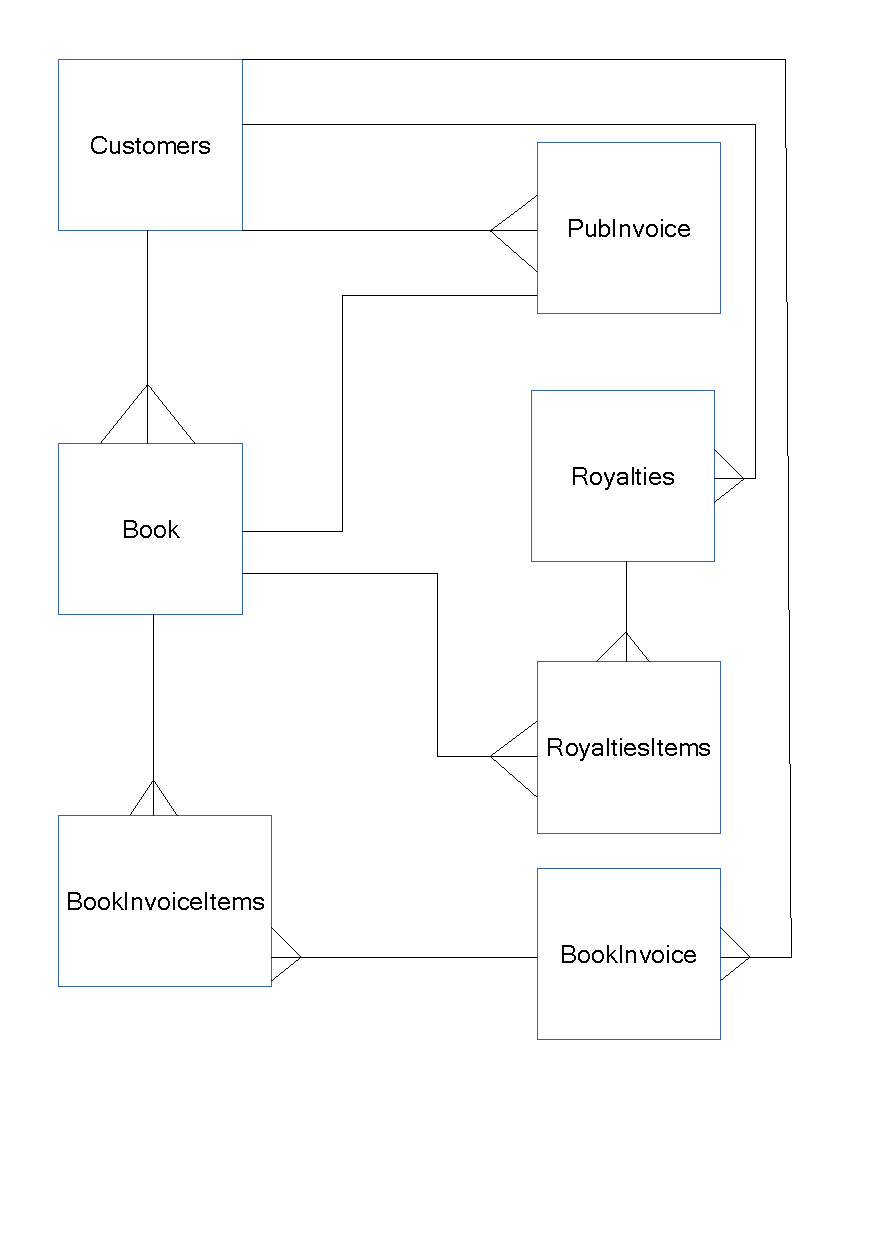
\includegraphics[width=\textwidth]{./Design/ER_Diagram.pdf}
\end{figure}


\subsubsection{Entity Descriptions}

Customer(\underline{Author ID}, FirstName, LastName, Email, Address, Postcode, Phone Number)

Invoice(\underline{InvoicePayment}, \underline{InvoiceDate}, \emph{ISBN}, \emph{AuthorID}, InvoiceQuantity, InvoiceDiscount, ShippingPrice, ShippingType)

Royalties(\underline{RoyaltyPayment}, \underline{RoyaltiesDate}, \emph{ISBN}, \emph{AuthorID}, RoyaltyDiscount, WholeSalePrice, RoyaltyQuantity, NetSales, PrintCost)

Book(\underline{ISBN}, \emph{AuthorID}, Book Title, NoOfPages, Size, Cover, Paper, Back, Paper, Font, FontSize, DatePublished, Price)

\subsubsection{UNF to 3NF}

Key:

\textbf{Bold Font} = Primary Key

\emph{Italics} = Foreign Key

Each Column represents a new group.

\newpage
First of all, I have started with the data in its unnormalised form.

\begin{tabular}{|p{3.5cm}|}
    \hline
    FirstName \\
    LastName \\
    Email \\
    PhoneNumber \\
    Address \\
    PostCode \\
    AuthorID \\
    ISBN \\
    BookTitle \\
    NoOfPages \\
    Size \\
    Back \\
    Cover \\
    Paper \\
    Font \\
    FontSize \\
    DatePublished \\
    Price \\
    RoyaltiesID \\
    RoyaltiesItems \\
    Currency \\
    RoyaltyPayment \\
    RoyaltiesDate \\
    RoyaltyDiscount \\
    WholeSalePrice \\
    RoyaltyQuantity \\
    NetSales \\
    PrintCost \\
    ExcRateToGBP \\
    PubInvoiceID \\
    PubInvoicePayment \\
    PubInvoiceDate \\
    PubInvoiceService \\
    PubInvoiceOrder \\
    BooksInvoiceID \\
    BooksInvoiceItems \\
    BooksInvoicePayment
    BooksInvoiceDate \\
    BooksInvoiceDiscount \\
    BooksInvoiceQuantity \\
    ShippingType \\
    ShippingPrice \\
    \hline
\end{tabular}

\newpage
Then, I put it into the first normal form.

\begin{tabular}{|p{2.5cm}|p{3.5cm}|}
    \hline
    \textbf{AuthorID} & \textbf{ISBN} \\
    FirstName & \textbf{AuthorID} \\
    LastName & BookTitle \\
    Email & NoOfPages \\
    PhoneNumber & Size \\
    Address & Back \\
    PostCode & Cover \\
    & Paper \\
    & Font \\
    & FontSize \\
    & DatePublished\\
    & Price \\
    & RoyaltiesID \\
    & RoyaltiesItems \\
    & Currency \\
    & RoyaltyPayment \\
    & RoyaltiesDate \\
    & RoyaltyDiscount \\
    & WholeSalePrice \\
    & RoyaltyQuantity \\
    & NetSales \\
    & PrintCost \\
    & ExcRateToGBP \\
    & PubInvoiceID \\
    & PubInvoiceDate \\
    & PubInvoiceService \\
    & PubInvoiceOrder \\
    & PubInvoicePayment \\
    & BooksInvoiceID \\
    & BooksInvoiceItems \\
    & BooksInvoicePayment \\
    & BooksInvoiceDate \\
    & BooksInvoiceDiscount \\
    & BooksInvoiceQuantity \\
    & ShippingType \\
    & ShippingPrice \\
    \hline
\end{tabular}

\newpage
After that, I put it into the second normal form.

\begin{tabular}{|p{2.5cm}|p{3.5cm}|p{2.5cm}|}
    \hline
    \textbf{AuthorID} & \textbf{ISBN} & \textbf{ISBN} \\
    FirstName & \textbf{AuthorID} & BookTitle \\
    LastName & RoyaltiesID & NoOfPages \\
    Email  & Currency & Size \\
    PhoneNumber & RoyaltyPayment & Back \\
    Address & RoyaltiesDate & Cover \\
    PostCode & RoyaltyDiscount & Paper \\
    & WholeSalePrice & Font \\
    & RoyaltyQuantity & FontSize \\
    & NetSales & DatePublished \\
    & PrintCost & Price \\
    & ExcRateToGBP & \\
    & PubInvoiceID & \\
    & PubInvoiceDate & \\
    & PubInvoiceService & \\
    & PubInvoiceOrder & \\
    & PubInvoicePayment & \\
    & BooksInvoiceID & \\
    & BooksInvoiceItems & \\
    & BooksInvoicePayment & \\
    & BooksInvoiceDate & \\
    & BooksInvoiceDiscount & \\
    & BooksInvoiceQuantity & \\
    & ShippingType & \\
    & ShippingPrice & \\
    \hline
\end{tabular}

\newpage
Finally, I put the data into its third normal form.

\begin{tabular}{|p{2.5cm}|p{2.5cm}|p{2.5cm}|p{3cm}|p{3cm}|}
    \hline
    \textbf{AuthorID} & \textbf{ISBN} & \textbf{RoyaltiesID} & \textbf{RoyaltiesItems} & \textbf{PubInvoiceID} \\
    FirstName & \emph{AuthorID} & \emph{AuthorID} & \emph{RoyaltiesID} & \emph{AuthorID} \\
    LastName & BookTitle & \emph{ISBN} & Currency & \emph{ISBN} \\
    Email & NoOfPages & RoyaltyPayment & RoyaltyDiscount & PubInvoiceDate \\
    PhoneNumber & Size & RoyaltiesDate & WholeSalePrice & PubInvoiceService \\
    Address & Back & & RoyaltyQuantity & PubInvoiceOrder \\
    PostCode & Cover & & NetSales & PubInvoicePayment \\
    & Paper & & PrintCost & \\
    & Font & & ExcRateToGBP & \\
    & FontSize & & & \\
    & DatePublished & & & \\
    & Price & & & \\
    \hline
\end{tabular}

\begin{tabular}{|p{3.5cm}|p{3.5cm}|}
    \hline
    \textbf{BooksInvoiceID} & \textbf{BooksInvoiceItems} \\
    \emph{AuthorID} & \emph{BooksInvoiceID} \\
    BooksInvoicePayment & \emph{ISBN} \\
    BooksInvoiceDate & BooksInvoiceQuantity \\
    & BooksInvoiceDiscount \\
    & ShippingType \\
    & ShippingPrice \\
    \hline
\end{tabular}

\newpage
\subsection{SQL Queries}

I am using Python to format the SQL query text strings.

\begin{tabular}{|p{10cm}|p{5cm}|}
    \hline
    \textbf{SQL} & \textbf{Descriptions} \\ \hline 
     """insert into \\ Customer(FirstName, LastName, Email, PhoneNumber, Address, Postcode) values (\{0\}, \{1\}, \{2\}, \{3\}, \{4\}, \{5\}) \\ """.format(FirstName, LastName, Email, PhoneNumber, Address, Postcode) & An example of an SQL statement which adds customer records to the database. Here, it is entering a new customer record with the attributes: FirstName, LastName, Email, PhoneNumber, Address and Postcode. \\ \hline
    """create table RoyaltiesItems(\\ RoyaltiesID INTEGER, \\ Currency REAL, \\ RoyaltyDiscount STRING,\\  WholeSalePrice REAL,\\ RoyaltyQuantity INTEGER,\\ NetSales REAL,\\ PrintCost REAL, \\ ExcRateToGBP STRING \\ PRIMARY KEY(RoyaltiesItems) \\ FOREIGN KEY(RoyaltiesID) REFERENCES \\ Royalties(RoyaltiesID) """ & An example of an SQL statement that creates a new table for the Royalties. There is a primary key which is RoyaltiesItems, and there is one foreign key, which is RoyaltiesID. \\ \hline 
    """select Customer.LastName, Book.BookTitle \\ from Customer, Book \\ where Price < 13.00 and \\ Back = "Paperback"  & This statement will return all the LastNames and the BookTitles from the Customer table and the Book table whose book is paperback and costs less than £13. \\ \hline
\end{tabular}

\section{Security and Integrity of the System and Data}

\subsection{Security and Integrity of Data}

\subsection{System Security}

\section{Validation}

\section{Testing}

\begin{landscape}
\subsection{Outline Plan}

\begin{center}
    \begin{tabular}{|p{2cm}|p{5cm}|p{5cm}|p{4cm}|}
        \hline
        \textbf{Test Series} & \textbf{Purpose of Test Series} & \textbf{Testing Strategy} & \textbf{Strategy Rationale}\\ \hline
        Example & Example & Example & Example \\ \hline
    \end{tabular}
\end{center}

\subsection{Detailed Plan}

\begin{center}
    \begin{longtable}{|p{1.5cm}|p{2.5cm}|p{2.5cm}|p{2cm}|p{2cm}|p{2cm}|p{2cm}|p{2cm}|}
        \hline
        \textbf{Test Series} & \textbf{Purpose of Test} & \textbf{Test Description} & \textbf{Test Data} & \textbf{Test Data Type (Normal/ Erroneous/ Boundary)} & \textbf{Expected Result} & \textbf{Actual Result} & \textbf{Evidence}\\ \hline
        Example & Example & Example & Example & Example & Example & Example & Example \\ \hline
    \end{longtable}
\end{center}
\end{landscape}